\chapter{Boundary conditions}\label{lec:lec20}

At this point, we have quantities like charge density $\rho$\footnote[1]{$\rho$ is Rho, the 17th letter of the Greek alphabet}, volume density, conduction current density $\overline{J}$, displacement current density $\frac{\partial \overline{D}}{\partial t}$, surface charge density $\rho_s$ and then surface current density. So we can say these are the sources which are related to the fields (the electric and magnetic fields). In general, we can establish a relationship between these quantities which we can call the sources of the fields, and these relationships are called boundary conditions.

\section{Boundary Conditions}

We would now go back to the integral form of the maxwell's equations, take a sharp boundary media interface i.e where the medium property suddenly changes and then we establish a relationship between the electric and magnetic fields in the two regions. These boundary conditions are essential when we solve the electromagnetic problems in various media like coaxial cable, wave guides or optical fibre.

Whenever we solve the phenomenon of electromagnetics, generally these media constitute discrete boundaries and we require the relationship of electric and magnetic fields across this boundary called \textbf{Boundary Conditions}. These boundary conditions are essential in solving the electromagnetic problems in physical structures.

\subsection{Boundary Conditions 1 and 2}
Let us say we have a media interface and the two sides have different material properties i.e medium 1 with permittivity $\epsilon_1$, conductivity $\rho_1$ and permeability $\mu_1$, and medium 2 with $\epsilon_2$, $\rho_2$ and $\mu_2$ respectively. Now we can write the different integral equations in the form of maxwell's equation across the boundary. Consider a box and the boundary shown, if we apply Gauss's law across the boundary,
\begin{figure}[h]
\centering
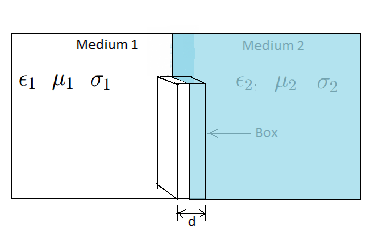
\includegraphics[width=1\linewidth]{./graphics/diemedium1}
\caption{A box in the boundary of two media.}
\end{figure}

According to Gauss's law, the total displacement coming out of the box is equal to the charges enclosed. If we make the thickness of the box shrink to zero. We will get a relationship between the displacement vector going in all directions as $d$ shrinks.  Let's say in medium 1 we have $D_{n1}$ and $D_{t1}$ as the normal and tangential components of the displacement vectors in medium 1 with respect to the surface of the box (Pillbox is the usual name). We have the figure below.
\begin{figure}[h]
\centering
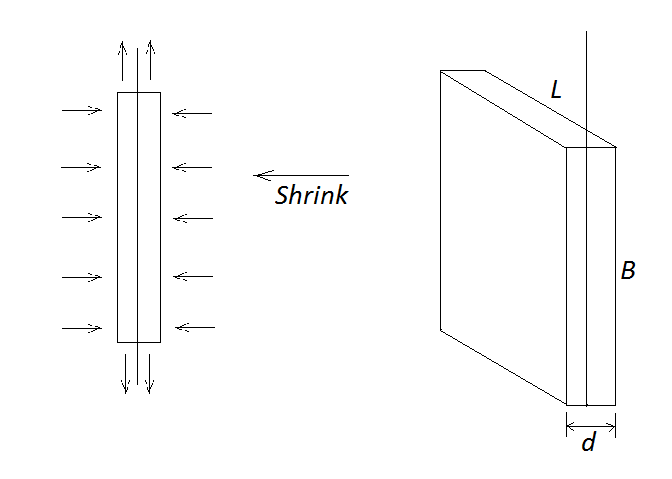
\includegraphics[width=.7\linewidth]{./graphics/diemedium2}
\caption{Shrinking box.}
\end{figure}

Any general displacement vector in medium 1 close to the interface can be resolved into two components, the tangential $D_{t1}$ and normal components $D_{n1}$. 
\begin{figure}[h]
\centering
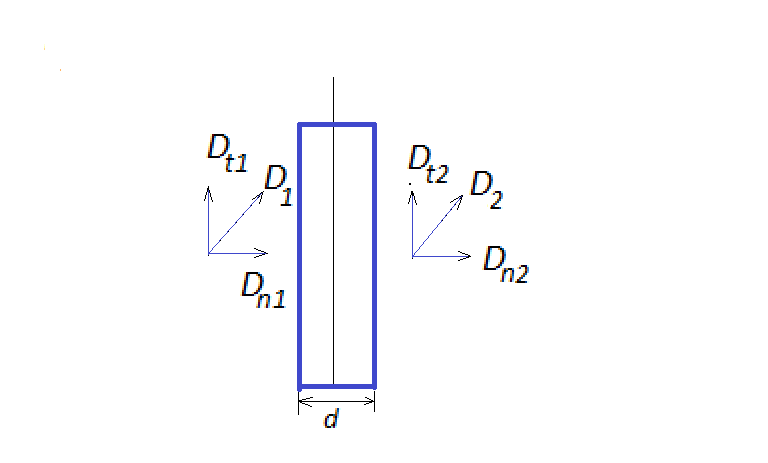
\includegraphics[width=1\linewidth]{./graphics/diemedium3}
\caption{Normal and tangential components of Displacement vector $\overline{D}$.}
\end{figure}
Similarly, for medium 2 the tangential and normal components are $D_{t2}$ and $D_{n2}$ respectively. The normal displacement coming from the box when the thickness of the box tends to zero i.e $d \longrightarrow 0$, the displacement due to $D_{t1}$ and $D_{t2}$ becomes zero as the area on top and at the bottom becomes zero. So that the displacement coming out of the box with $d \longrightarrow 0$ is as a result of $D_{n1}$ and $D_{n2}$ only, as $L$ and $B$ are not affected by the shrinking. From Gauss's law, if we take a net normal displacement from the shrinked box, that will be equal to the total charge enclosed. With $d \longrightarrow 0$, this is nothing but the charge on the surface of the sheet (i.e the box which has now being compressed to the sheet) or Surface Charge.

The second possibility is that, if there is no charge enclosed at all (no surface charge) then $D_{n1}= D_{n2}$ since Gauss's law says that divergence of $\overline{D}$ should be zero, you have the continuity of the normal displacement vector $\overline{D}$.

So when 
$d \longrightarrow 0$ and there is a surface charge, $D_{n1}- D_{n2} = \rho_s$. But if there is no surface charge then $\rho_s = 0$ and $D_{n1}= D_{n2}$. So this is the boundary condition we have as a result of Gauss's law between two media. This is \textbf{Boundary condition 1}.


We can do the same thing for magnetic flux density also, i.e create the same box. But we see that there is nothing like net charge enclosed. That means that there is nothing like surface charge for magnetic field or $\rho_s = 0$. So the normal component of the magnetic flux density will always be continuous in the two media. This is \textbf{Boundary condition 2}. From Gauss's law, we have the boundary conditions.
\begin{enumerate}[(i)]
\item Normal component of $\overline{D}$ is continuous if no surface charge is present. In the presence of surface charge $\rho_s$, $D_{n1}- D_{n2} = \rho_s$.
\item Normal component of $\overline{B}$ is continuous i.e $B_{n1} = B_{n2}$.
\end{enumerate}

We now have the boundary conditions on the displacement vector $\overline{D}$ and the magnetic flux density $\overline{B}$. Magnetic flux density satisfy the condition that the normal component is always continuous whatever the media discontinuities are. Whereas the displacement vector if there are surface charges  is $D_{n1}- D_{n2} = \rho_s$ or $D_{n1} = D_{n2} $ if $\rho_s = 0$. 
\subsection{Boundary Conditions 3 and 4.}
By using Ampere's circuit law and the Faraday's laws, we will get two more boundary conditions on the electric and magnetic fields. Let us take a dielectric medium, we have tangential and normal components of electric field given as $E_{t1}$ and $E_{t2}$, and in medium 2 we have $E_{t2}$ and $E_{n2}$ respectively.

If we take a loop around the boundary
\begin{figure}[h]
\centering
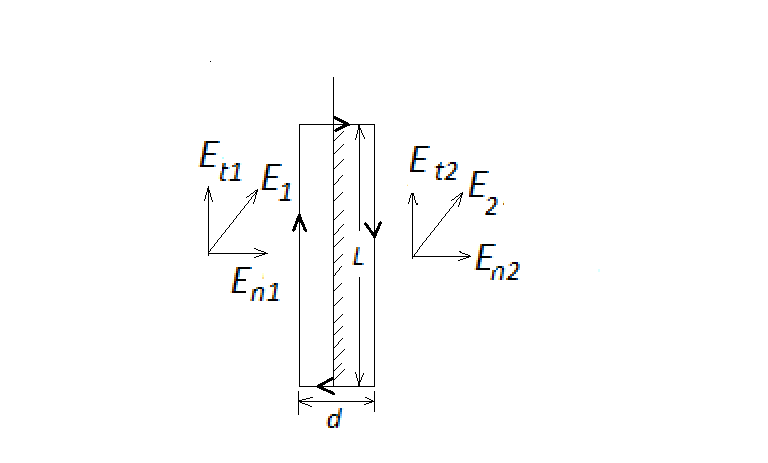
\includegraphics[width=1\linewidth]{./graphics/diemedium4}
\caption{Boundary loop.}
\end{figure}
(not a box this time) and then apply Faraday's law across the loop, then find the line integral to get electromotive force emf, it must be equal to the rate of change of flux in that loop. Since we are talking about a finite magnetic flux density $\overline{B}$i.e the rate of change of flux in that loop is also a finite quantity. $\overline{E}.\overline{dl} = 0$ for $E_{n1}$ and $E_{n2}$ only. $E_{t1}$ and $E_{t2}$ will contribute when $L \longrightarrow 0$. 

As $E_{n1}d$ and $E_{n2}d\longrightarrow 0$ with $d \longrightarrow 0$. So we get 
\begin{align*}
E_{t1}L - E_{t2}L = 0
\end{align*}
as 
\begin{align*}
\frac{\partial}{\partial t}(\phi) = \frac{\partial}{\partial t}(BA
)
\end{align*}
$A =  Area\ of\ the\ loop$, and this area becomes zero as the loop shrinks to a line element with $d = 0$. So when the loop shrinks to a thin sheet, the line integral contribution from top to bottom of the loop goes to zero, so we only have contribution to this integral from left and right side as a result of $E_{t1}$ and $E_{t2}$. So, 
\begin{align*}
E_{t1}L + E_{n1}d +E_{t2}(-L) + E_{n2}(-d) = 0
\end{align*}
but $E_{n1}d$ and $E_{n2}d = 0$ since $d \longrightarrow 0$, so that 
\begin{align*}
E_{t1}L - E_{t2}L = 0 = \frac{\partial}{\partial t}(BA)
\end{align*}
Hence,
\begin{align*}
E_{t1} = E_{t2}
\end{align*}
Therefore, the tangential component of electric field is continuous across the boundary irrespective of what the boundary condition is, the tangential component of the electric field will always be continuous across the boundary. This is because the magnetic flux density is always finite in the region enclosed by the loop. This is \textbf{Boundary Condition 3}. 

The same can be done for the Ampere's circuit law for the magnetic fields in medium 1 as $H_{t1}$, $H_{n1}$ and $H_{t2}$, $H_{n2}$ for medium 2 respectively. We apply Ampere's law around the loop.
\begin{figure}[h]
\centering
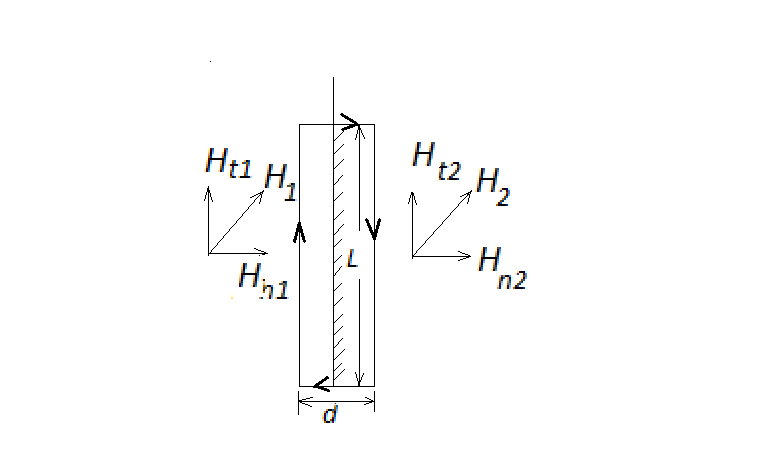
\includegraphics[width=1\linewidth]{./graphics/diemedium4_2}
\caption{Ampere's law is applied around the loop.}
\end{figure}
This we do by finding the line integral of $H$ around the loop (magnetomotive force) in a clockwise direction. Even if $\frac{\partial\overline{D}}{\partial t}$ ( displacement current density) was available and perpendicular to the plane of $Ld$ outward, $\frac{\partial\overline{D}}{\partial t}. Ld$ will give current, but with finite current density and area $Ld$ going to zero,  $\frac{\partial\overline{D}}{\partial t}. Ld \rightarrow 0 $. So,
\begin{align*}
(H_{t1} - H_{t2})L = J.A +\frac{\partial D}{\partial t}.A
\end{align*}
Another possibility is, we may have sufficient current $J_s$ on the $Ld$ plane, but when the loop area tends to zero ($d \rightarrow 0 $), the surface current $J_s$ is still available . So we can have the equation below accounting for all possible current sources, in this case magnetic field.
\begin{equation}
(H_{t1} - H_{t2})L = J.A +\frac{\partial D}{\partial t}.A + J_sL
\end{equation}
with $A \rightarrow 0$
\begin{align*}
(H_{t1} - H_{t2})L = J_sL
\end{align*}
Hence, the difference of the tangential component of the magnetic fields multiplied by the loop length $L = suface\ current\ density \times L$ . Therefore,
\begin{equation}
H_{t1} - H_{t2} = J_s
\end{equation}
If there is no surface current density, then 
\begin{equation}
H_{t1} = H_{t2}
\end{equation}
i.e the tangential component of the magnetic field is continuous between the boundary if there is no surface current density.

Using the four Maxwell's equations in integral form for two media interface, we get the so called boundary conditions. What we have done is to start with the four basic laws in integral form and we convert to differential form using Stoke's and divergence theorems. We had Maxwell's equations in both integral and differential forms. The differential form of Maxwell's equations are the point relations.

However, the differential form cannot be used in situations where you have media discontinuities because they require space derivatives and at discontinuity, these space derivative is undefined. In these cases, we apply the integral form. When we apply the integral form to the media interfaces, we get the boundary conditions. With $\overline{H}_1$ and $\overline{H}_2$ shown in the figure below.
\begin{figure}[h]
\centering
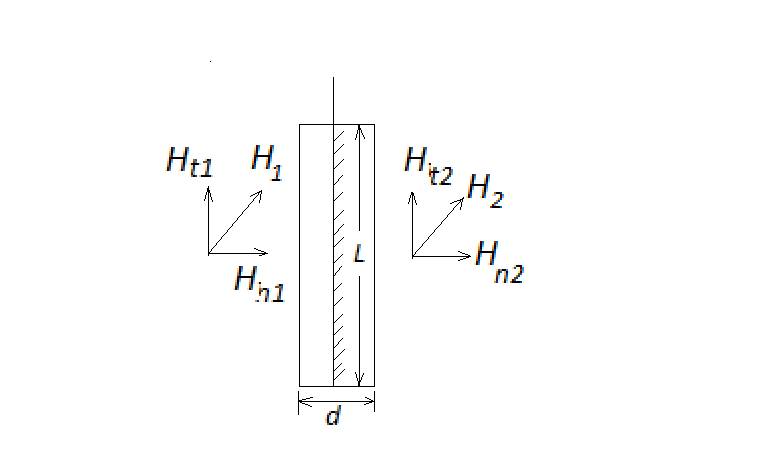
\includegraphics[width=1\linewidth]{./graphics/diemedium4_2_2}
\caption{Boundary with normal and tangential components of magnetic field intensity $\overline{H}$ shown.}
\end{figure}

We can rewrite 
\begin{equation*}
H_{t1} - H_{t2} = J_s
\end{equation*}
as
\begin{equation}
\hat{n} \times (\overline{H}_1 - \overline{H}_2) = \overline{J}_s\hat{n}
\end{equation}
This is \textbf{Boundary Condition 4}. The cross product of $\hat{n}$ and $\overline{H}$ gives you the tangential component. Recall the definition of cross product,
\begin{equation*}
\overline{a}\times\overline{b} = \left|a \right| \left|b \right|sin\theta 
\end{equation*}
with $\overline{a} = \hat{n}$ and $ b = \overline{H}_1$
\begin{align*}
&\hat{n}\times\overline{H}_1 = \left|H_1 \right|sin\theta = H_{t1} \\ because\ the\ & magnitude\ of\ \hat{n}\ is\ unity\ i.e\ 1.
\end{align*}
With this we can summarize the four boundary conditions for the dielectric media as we have been discussing. We will do this in the next section.
\section{Dielectric - Dielectric Interface}
When we have a medium on both sides of a dielectric.
\begin{figure}[h]
\centering
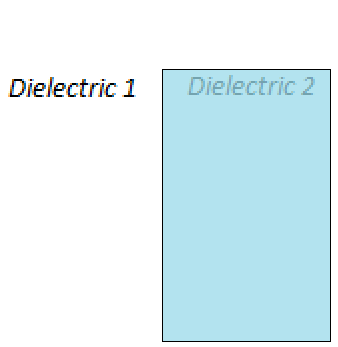
\includegraphics[width=.6\linewidth]{./graphics/diemedium5}
\caption{Dielectric - Dielectric boundary Interface.}
\end{figure}

The conductivity may be finite or even zero, but the conductivity is not infinite. This means there is no conductor on either side of the boundary. In that case we have the following boundary conditions.
\begin{enumerate}[(i)]
\item $D_{n1} - D_{n2} = \rho_s$
\item $B_{n1} = B_{n2}$
\item $E_{t1} = E_{t2}$
\item $\hat{n} \times (\overline{H}_2 - \overline{H}_1) = \overline{J}_s$
\end{enumerate}

Conditions (ii) and (iii) can be applied whether you have surface charge or current. (i) and (iv) may be continuous if $\rho_s = \overline{J}_s = 0$ but may not be continuous if $\rho_s\neq 0$ and $\overline{J}_s\neq 0$.
Therefore, unless we have a knowledge of surface charge $\rho_s$ or surface current $\overline{J}_s$, the boundary condition 1 and 4 may not easily be applied, but 2 and 3 can easily be applied because they do not require the knowledge of surface charge or current.

\section{Dielectric - Conductor Interface}
We would now take a dielectric to conducting media. This is what we have in transmission structures like coaxial cables, waveguides and transmission lines. We would like to find the boundary conditions to the dielectric to conducting media. 
\begin{figure}[h]
\centering
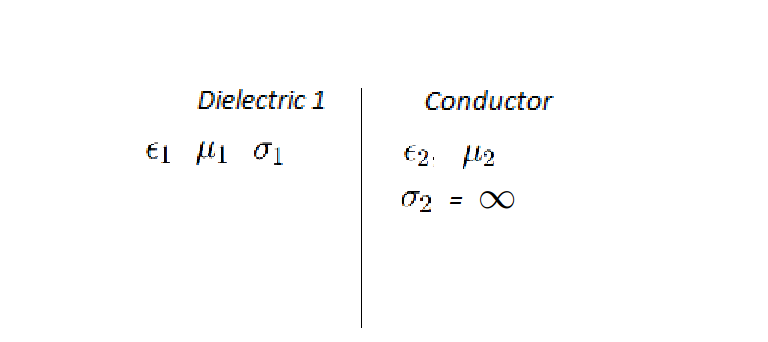
\includegraphics[width=1\linewidth]{./graphics/diemedium5_2}
\caption{Dielectric - Conductor Interface.}
\end{figure}

First, we note that if we have one of the medium as a  conductor with infinite conductivity and we want to find the current densities, the current density is 
\begin{equation}
\overline{J} = \sigma\overline{E}
\end{equation}
since $\sigma$ is infinite and $\overline{E}$ finite,
\begin{equation*}
\overline{J} = \infty\overline{E}
\end{equation*} 
then,
\begin{align*}
\overline{J} = \infty
\end{align*}
in the conductor medium. From the expressions above, if we say we have a finite current densities for ideal conductors, the electric field $\overline{E}$ must be ideally zero. Because,
\begin{align*}
\frac{\overline{J}}{0} = \infty
\end{align*}
Otherwise, for even arbitrarily small values of electric field $\overline{E}$, the conduction current density will be infinite in the conductor medium. That is the reason when conductivity tends to infinity, the electric field in the conducting medium must tend to zero. Also, we have seen from Maxwell's equations that the electric field is related to the magnetic field and vice versa. 

So if we have a time varying electric field which is identically zero in the conductor medium, then the magnetic field will be zero in that region. So ideal conductors do not have magnetic field inside the conductor medium. However, imagine a situation where we apply a small arbitrary value of electric field which is in the direction perpendicular to the interface. it will drive the charges inside the conductor to the surface. It means we can have accumulation on the surface of the of the conductor. 

Similarly, it is possible that when we have time varying fields, there might be current flowing across the surface of the conductor. Therefore, for an ideal conductor the field inside it is zero, but we can have surface charges and surface current. The situation is as we have it in the figure below.
\begin{figure}[h]
\centering
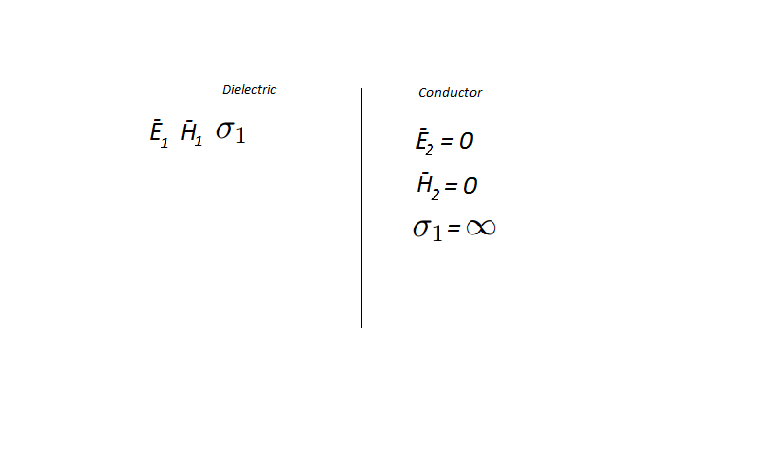
\includegraphics[width=1\linewidth]{./graphics/diemedium5_2_2}
\caption{Dielectric - Conductor Interface.}
\end{figure}

Now, with $\overline{E}_2 = 0$ and $\overline{H}_2 = 0$ for the conducting medium, we go back to apply the boundary conditions.
\begin{equation*}
\overline{D}_{n2} = 0\quad since\quad \overline{D}_{n2} = \epsilon\overline{E}_{n2}
\end{equation*}
So,
\begin{align*}
D_{n1} &= \rho_s \\
B_{n1} &= 0 \\
E_{t1} &= 0 \\
\hat{n}\times\overline{H}_1 &= \overline{J}_s
\end{align*}
If $\rho_s = J_s = 0$, then
\begin{align*}
\overline{D}_{n1} = 0\quad and \quad -\hat{n}\times\overline{H}_{1} = 0
\end{align*}
So, depending on the situation whether we have dielectric to dielectric interface or dielectric to conductor interface, we apply the appropriate boundary conditions. This gives us the framework for analyzing any electromagnetic problem in three dimensional space. 

In summary, starting from the basic laws, we found out Maxwell's equations. We are now going to make use of Maxwell's equation in integral form to analyze electromagnetic problem in three dimensional space. We got boundary conditions which will be useful when we try to solve the electric and magnetic fields across dielectric - dielectric or dielectric - conductor interfaces. Let us now solve some problems to reinforce these concepts as it relates to time varying charges and time varying fields.
\begin{exmp}
Two charges $Q_A$ and $Q_B$ are separated by a distance of 10m. $Q_A = 10cos\omega t$ and $Q_B = -10cos\omega t$, $\omega = 10^3 rad/s$. Find the magnetic flux density at a point which is at a distance of 10m from both charges.

\subsubsection*{Solution}
Let P be the point at which to find $\overline{E}$. At $t = 0$, $Q_A = +10C$ and $Q_B = -10C$ and that shows the direction of the $\overline{E}$ field also by $\overline{E}_{A}$ and $\overline{E}_{B}$. Let $Q_A$ and $Q_B$ lie on the $Z$ axis as shown .
\begin{figure}[h]
\centering
% \includegraphics[width=1\linewidth]{./graphics/fig2010}
\caption{Diagram showing charges $Q_A$, $Q_B$ and point $P$.}
\end{figure}

\begin{align*}
E_A &= \frac{10cos\omega t}{4\pi\epsilon_or^2}\\
E_B &= \frac{-10cos\omega t}{4\pi\epsilon_o r^2}
\end{align*}
$E_A$ and $E_B$ are same in magnitude and are resolved into $E_T$
\begin{align*}
E_T &= E_Asin\theta - E_Bsin\theta = \frac{20cos\omega t}{4\pi\epsilon_o r^2} \\
since \theta &= \frac{5}{10} = \frac{1}{2}, \quad \theta = \angle {30} \ or \ \frac{\pi}{6}
\end{align*}
\begin{align*}
E_T = \frac{-20cos\omega t}{4\pi\epsilon_o r^2}\hat{z}.\frac{1}{2} = \frac{-10cos\omega t}{4\pi\epsilon_o r^2}\hat{z}
\end{align*}
Now we know the total magnetic field, we can apply Maxwell's equation and find out the magnetic field due to the charges.
\begin{align*}
\overline{H} = \frac{-1}{\jmath\omega\mu_o}\nabla\times\overline{E}
\end{align*}
and,
\begin{align*}
\nabla\times\overline{E} = \frac{-\partial\overline{B}}{\partial t} = \frac{-\partial}{\partial t}(\mu_o\overline{H})
\end{align*}
or,
\begin{align*}
\overline{H} = \frac{-1}{\mu_o}\int(\nabla\times\overline{E})dt
\end{align*}
\begin{align*}
\overline{E} = \frac{-10}{4\pi\epsilon_o r^2}Re(e^{\jmath\omega t})
\end{align*}
\begin{align*}
\overline{H} &= \frac{-1}{\mu_o}\int(\nabla\times\overline{E})dt = \frac{-1}{\mu_o}Re\nabla\times\int\overline{E}dt\\
&= \frac{-1}{\mu_o}Re\nabla\times\int\frac{-10}{4\pi\epsilon_o r^2}e^{\jmath\omega t}dt\hat{z}
\end{align*}
\begin{dmath*}
\overline{H} = \frac{-1}{\mu_o}\nabla\times Re\left[\frac{1}{\jmath\omega}Ke^{\jmath\omega t} \right]\hat{z}\quad with\quad K =\frac{-10}{4\pi\epsilon_o r^2}
=\frac{-1}{\mu_o}\nabla\times Re\left[\frac{1}{\jmath\omega}(kcos\omega t + \jmath Ksin\omega t)\hat{z} \right]
= \frac{-1}{\mu_o}\nabla\times Re\left(\frac{kcos\omega t}{\jmath\omega} + \frac{ksin\omega t}{\omega} \right)\hat{z}
= \frac{-1}{\mu_o} \nabla\times\left(\frac{ksin\omega t}{\omega} \right)\hat{z}
= \frac{-1}{\mu_o\omega}\nabla\times\left(\frac{-10sin\omega t}{4\pi\epsilon_o r^2} \hat{z}\right)=\frac{-1}{\mu_o\omega}\begin{vmatrix}
\hat{x} &\hat{y} &\hat{z}\\
\frac{\partial}{\partial x} & \frac{\partial}{\partial y} & \frac{\partial}{\partial z} \\
0 &0 &\frac{-10sin\omega t}{4\pi\epsilon_o r^2}
\end{vmatrix}
= \frac{-1}{\mu_o\omega}\left[\left[  0 - \frac{\partial}{\partial x}\left( \frac{-10sin\omega t}{4\pi \epsilon_o r^2}\right)  \right]\hat{y} + \left[ \frac{\partial}{\partial y}\left(\frac{-10sin\omega t}{4 \pi\epsilon_o r^2} \right)\hat{x}\right]\right] 
\end{dmath*}
$r = \sqrt{Z^2 + x^2}$,therefore
\begin{align*}
\frac{\partial }{\partial x}\left(\frac{1}{r^2} \right) &=  \frac{\partial }{\partial x}\left(\frac{1}{Z^2 + x^2} \right)\\
&= \frac{-2x}{(Z^2 + x^2)^2} = \frac{-2x}{r^4} 
\end{align*}
but,
\begin{align*}
\frac{\partial}{\partial y}\left(\frac{1}{r^2} \right) = \frac{\partial}{\partial y}\left(\frac{1}{Z^2 + x^2} \right) = 0  
\end{align*}
\begin{align*}
\overline{H} &= \frac{-1}{\mu_o\omega}\left[ \frac{10sin\omega t}{4\pi\epsilon_o}.\frac{-2x}{r^4}\right]\hat{y} \\
&= \frac{1}{\mu_o\omega}\left[ \frac{20sin\omega t}{40000\pi\epsilon_o}x\hat{y}\right] \ because\ r = 10m 
\end{align*}
and
\begin{align*}
x = \sqrt{100 - 25} = 5\sqrt{3}
\end{align*}
so
\begin{align*}
\overline{H} &=  \frac{100\sqrt{3}sin\omega t}{40000\pi\epsilon_o\mu_o\omega}\hat{y}\\
&= \frac{3sin\omega t}{400\sqrt{3}\pi\epsilon_o\mu_o\omega}\hat{y} \\
&= \frac{3\sqrt{3}sin\omega t}{1200\pi\epsilon_o\mu_o\omega}
\end{align*}
\end{exmp}

From this, we see that when we have a time varying charge, they produce electric and magnetic fields and as we have seen from Maxwell's equations. Whenever we have time varying fields, electric and magnetic fields coexist.

Let us consider a problem based on the boundary conditions. Boundary condition is nothing but application of Maxwell's equation in integral form across a boundary. It means if the laws are expressed in differential form, we get the point form of Maxwell's equation.
\begin{exmp}
A medium has infinite conductivity for $Z<0$, and $E_r=5$, $\mu_r = 20$, $\sigma = 0$ for $Z>0$. If the electric field for $Z>0$ is given by 
\begin{align*}
\overline{E} = 10cos(3\times 10^8t - 10x)\hat{z}
\end{align*}
Find the surface charge density and the surface current density at the location (2,3,0) at the time $t = 0.5nsec$.\\
\subsubsection*{Solution}
With infinite conductivity for $Z>0$, that is an ideal conductor, electric and magnetic field cannot exist inside it. Electric field is normal to the surface as shown in the diagram.
\begin{figure}[h]
\centering
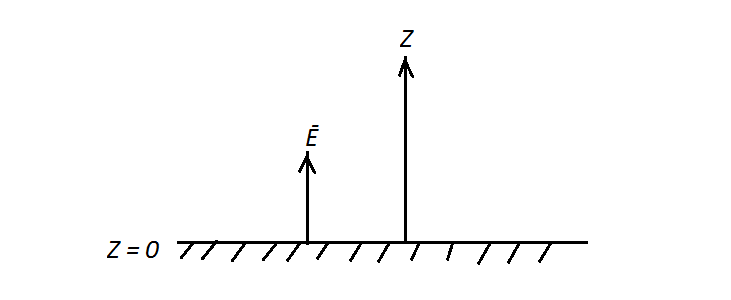
\includegraphics[width=1\linewidth]{./graphics/diemedium7}
\caption{Medium with electric field $\overline{E}$ and conductivity Z direction shown.}
\end{figure}

The surface charge density in this case is $\rho_s = \epsilon_o\epsilon_rE_n$
\begin{align*}
\rho_s = \epsilon_o(5)10cos(3\times10^8t - 10x)
\end{align*}
Substituting location (2,3,0) at x = 2m and $t = 0.5\times 10^-9sec$,
\begin{dmath*}
\rho_s = \epsilon_o(5)10cos(3\times 10^8\times 0.5\times10^{-9} - 10\times 2) = 2.389\times 10^-11 C/m^2
\end{dmath*}
Next we find the surface current density at that location. As we know, for a conducting boundary, the surface current density is related to the magnetic field. \\
So, if we know the tangential component of the magnetic field at the conducting boundary, then we can find out what is the surface current at that boundary. We use the curl equation to find out what will be the magnetic field on the surface of the boundary. So,
\begin{align*}
\nabla\times \overline{E} = \begin{vmatrix}
\hat{x} &\hat{y} &\hat{z}\\
\frac{\partial}{\partial x} & \frac{\partial}{\partial y} & \frac{\partial}{\partial z} \\
0 &0 &E_z
\end{vmatrix}
\end{align*}
From Faraday's law,
\begin{align*}
\nabla\times\overline{E} = -\mu_o\mu_r\frac{\partial\overline{H}}{\partial t}
\end{align*}
\begin{align*}
\overline{H} = \frac{1}{-\mu_o\mu_r}\int (\nabla\times\overline{E})dt
\end{align*}
But E is only a function of x, then
\begin{dmath*}
\frac{\partial E_z}{\partial y} = 0,\quad \frac{\partial E_z}{\partial x} = \frac{\partial}{\partial x}\left[ 10cos(3\times 10^8 - 10x) \right] = -100cos(3\times 10^8 t - 10x)
\end{dmath*}
\begin{align*}
\nabla\times\overline{E} = \frac{-\partial E_z}{\partial x}\hat{y} = -100cos(3\times10^8t - 10x)\hat{y}
\end{align*}
Substituting into the $\overline{H}$ expression,
\begin{align*}
\overline{H} &= \frac{-1}{\mu_o\mu_r}\int-100cos(3\times 10^8t - 10x)\hat{y}dt \\
&=\frac{100}{\mu_o\mu_r}\int cos(3\times 10^8t - 10x)\hat{y}dt \\
&=\frac{100}{3\times 10^8}sin(3\times 10^8t - 10x)\hat{y}\\
\overline{H} &= \frac{100}{\mu_o\mu_r}\frac{sin(3\times 10^8t -10x)}{3\times 10^8}\hat{y} A/m
\end{align*}
Now we have a magnetic field which is $y$ oriented, so the $y$ oriented magnetic field is now tangential to the surface of the conducting boundary. We can find $\nabla\times\overline{H}$ to get the surface current as
\begin{dmath*}
Surface\ current,\quad \overline{J}_s = \hat{n}\times\overline{H} = \hat{z}\times \left\lbrace \frac{100}{\mu_o\mu_r}\frac{sin(3\times 10^8t -10x)}{3\times 10^8}\hat{y} \right\rbrace  
\end{dmath*}
But, $\hat{z}\times\hat{y} = -\hat{x}$
\begin{align*}
\overline{J}_s = \frac{-100}{\mu_o\mu_r}\frac{sin(3\times 10^8t -10x)}{3\times 10^8}\hat{x} A/m
\end{align*}
The surface current density at (2,3,0) which is at x = 2m and t = 0.5ns.
\begin{dmath*}
\overline{J}_s = \frac{100}{\mu_o\mu_r}\frac{sin(3\times 10^8\times 0.5 \times 10^{-9} - 10\times 2)}{3\times 10^8}\hat{x} = 1.116\times 10^{-2} A/m
\end{dmath*}
\end{exmp} 
Here's what we did. From the knowledge of electric field we found out the magnetic field. We then found out the tangential component of the magnetic field. Then, using the boundary condition $\hat{n}\times\overline{H} = \overline{J}_s$, we found out the surface current on the conducting boundary and at location $x = 2m$ and $t = 0.5nsec$. Finally, we found the surface current on the conducting boundary.

For time varying cases, one can specify either the electric field or the magnetic field near the conducting boundary or dielectric boundary and then by applying the same physical laws in the integral form and applying boundary conditions, we can get the quantities on the surface.
